\documentclass[12pt,a4paper]{scrartcl}
\usepackage{tikz}
\usepackage{listings}
\lstset{
language=python,
keywordstyle=\ttfamily\color{red}\bfseries,
backgroundcolor=\color{blue!15},
numbers=left,
}
	
\begin{document}

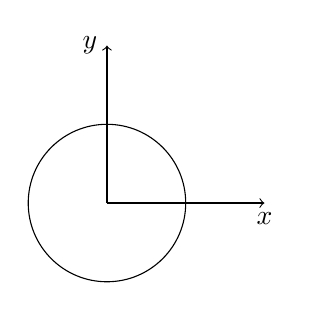
\begin{tikzpicture}
\draw[->] (0, 0) -- (2,0)node[below]{$x$};
\draw[->] (0, 0) -- (0,2)node[left]{$y$};
\draw (0, 0) circle(1);
\end{tikzpicture}

\begin{lstlisting}
f = lambda x: x**2 
g = lambda y: y//2
\end{lstlisting}
\end{document}	